\documentclass[11pt]{article}
\usepackage[utf8]{inputenc}
\usepackage{graphicx}
\usepackage{amsmath}
% --- Algorithms ---
\usepackage{algorithm}
\usepackage{algpseudocode}
\usepackage{subcaption} 

\title{Aberration Correction using Zernike Polynomials}
\author{Sriram M}
\date{\today}

\begin{document}

\maketitle

\section{Introduction}

This contains on techniques to correct for aberrations using Zernike polynomials.

\section{Zernike Polynomials}   
Zernike polynomials are a sequence of orthogonal polynomials on the unit disk. They are used as basis functions to quantify aberrations.
Using the ansi index to order them  ${Z_n}$ represents the nth Zernike polynomial.

Any phase mask on a unit disk can be represented as a linear combination of Zernike polynomials.

\begin{equation}
    \phi(r,\theta) \;=\; \sum_{n=0}^{\infty} w_n \, Z_n(r,\theta).
\end{equation}
where \(w_n\) are the weights for each Zernike polynomial called Zernike coefficients. They are in units of radians of phase and can be converted to units of wavelengths.

\section{Aberration Correction}
We discuss two techniques to correct for aberrations using Zernike polynomials. 
Both techniques approximate the aberration phase profile for a tweezer or bottle beam using a linear combination of $n_{max}$ Zernike polynomials.

\begin{equation}
    \phi_{aberr,i}(r,\theta) \;=\; \sum_{n=0}^{n_{max}} w_{n,i} \, Z_n(r,\theta).
\end{equation}

\subsection{Iterative zernike perturbation (IZP)}
In this technique, we iteratively measure the optimal Zernike coefficients $w_{n,i}$ by perturbing each Zernike polynomial and measuring the Strehl ratio/ $R^2$/RMSE and correcting the aberration using Gerchberg Saxton Algorithm in Zernike Kernel Space.



\begin{algorithm}[H]
    \caption{Iterative Zernike Perturbation}
    \label{alg:izp_simple}
    \begin{algorithmic}[1]
    \State \textbf{for} $n = 0$ to $n_{\max}$ \textbf{do}
    \State \hspace{0.5cm} Step 1: Add $w_n \cdot Z_n$ to $\phi_{\text{tweezers}}$ for $w_n \in [-1, 1]$ in steps of $0.05$ (20 steps).
    \State \hspace{0.5cm} Step 2: For each tweezer ($i$) compute Strehl ratio ($S_{i,w_{n}}$) for each $w_n$.
    \State \hspace{0.5cm} Step 3: For each tweezer Fit a parabola to Strehl ratio vs. $w_n$ and find its maximum.  
    \State \hspace{0.5cm} Step 4: Use Gerchberg–Saxton algorithm in Zernike kernel space to compensate the aberration.  
    \State \textbf{end for}
\end{algorithmic}
\end{algorithm}

We repeat the above procedure for 4-5 iterations.\\






\begin{figure}[H]
    \centering
    % Row 1
    \begin{subfigure}{0.48\textwidth}
        \centering
        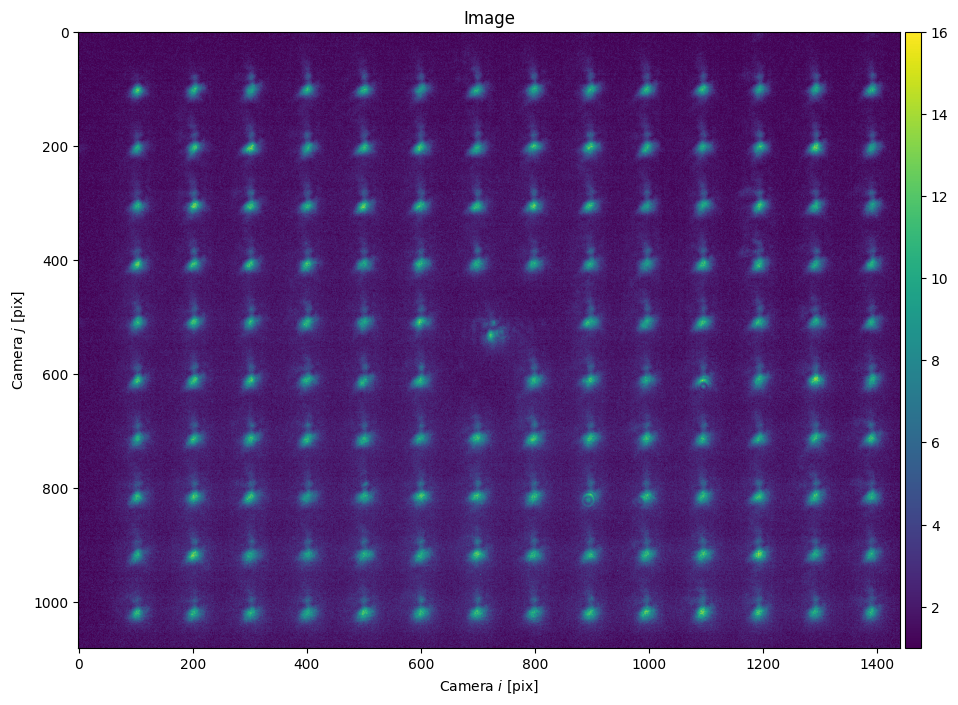
\includegraphics[width=\linewidth]{zernike_figures/izp_before.png}
        \caption{Without aberration correction.}
        \label{fig:izp_before}
    \end{subfigure}
    \hfill
    \begin{subfigure}{0.48\textwidth}
        \centering
        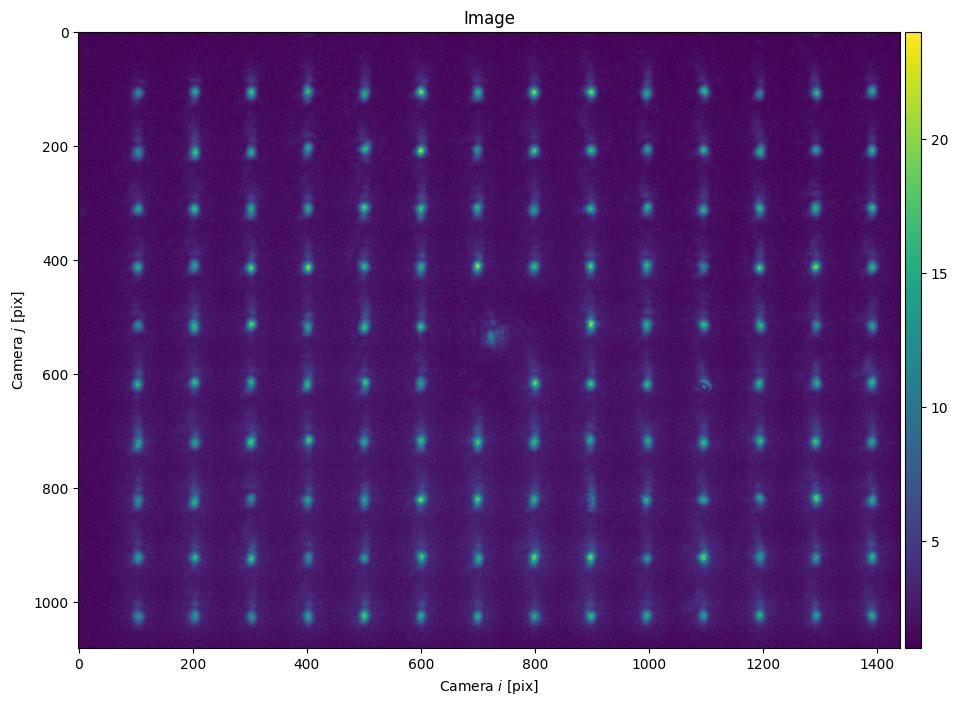
\includegraphics[width=\linewidth]{zernike_figures/izp_9.png}
        \caption{IZP with 9 Zernike terms.}
        \label{fig:izp_9}
    \end{subfigure}
    
    % Row 2
    \begin{subfigure}{0.48\textwidth}
        \centering
        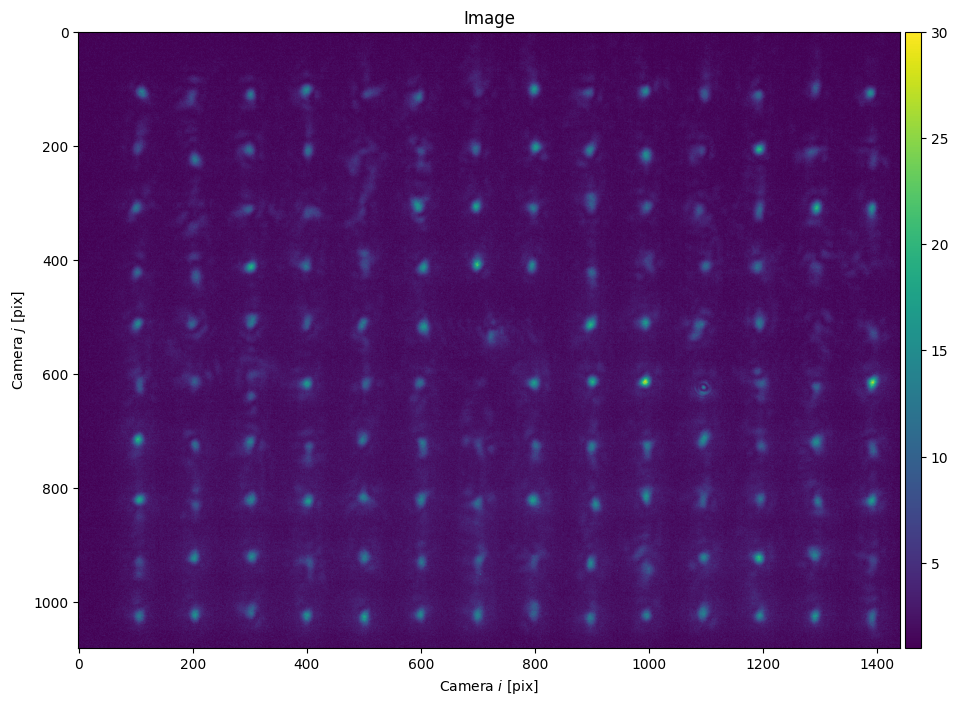
\includegraphics[width=\linewidth]{zernike_figures/izp_25.png}
        \caption{IZP with 25 Zernike terms.}
        \label{fig:izp_25}
    \end{subfigure}
    \hfill
    \begin{subfigure}{0.48\textwidth}
        \centering
        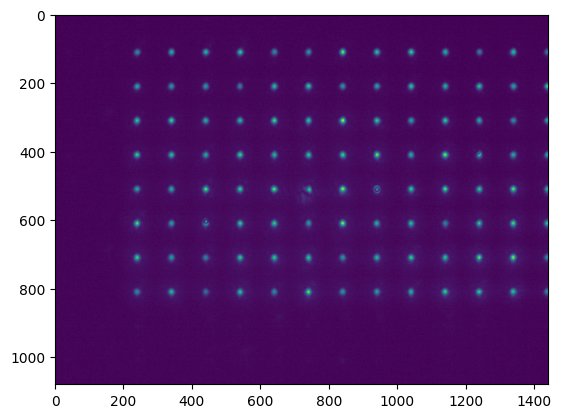
\includegraphics[width=\linewidth]{zernike_figures/sp.png}
        \caption{Superpixel aberration correction.}
        \label{fig:izp_sp}
    \end{subfigure}
    
    \caption{Comparison of aberration correction results with different methods. 
    (a) No correction, (b) IZP with 9 Zernike terms, (c) IZP with 25 Zernike terms, 
    and (d) superpixel aberration correction. The aberration correction is unstable especially for higher number of Zernike terms , and superpixel correction provides the best correction for our setup.}
    \label{fig:izp_comparison}
\end{figure}

This method worked somewhat for low order aberrations but is unstable escpecially for higher order aberrations as the number of Zernike polynomials increases and increasing no of iterations.
The authors mentioned the instability is due to the imperfect orthogonality of zernike modes.
For our setup, we found that superpixel based aberration correction worked better.\\

I tried this method over top of superpixel correction and it did not improve the results. Since the zernike coefficents are $<$ 0.2 after superpixel correction, the perturbations are too small to measure any change in Strehl ratio. The authors also claimed that they were able to converge the coefficents till  0.2

\begin{figure}[ht]
    \centering
    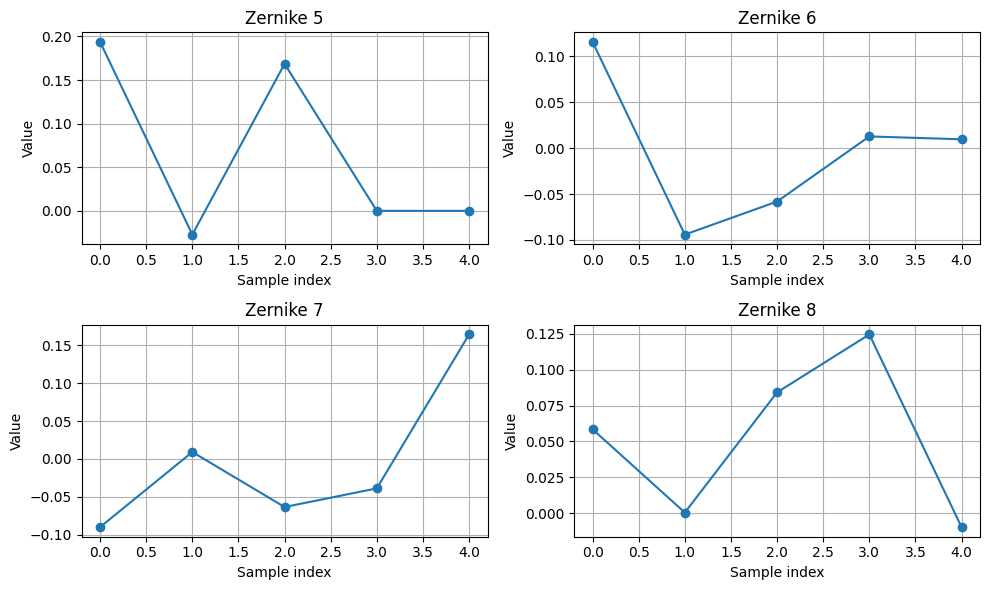
\includegraphics[width=0.85\textwidth]{zernike_figures/izp_sp.png}
    \caption{Evolution of selected Zernike coefficients across iterations during iterative Zernike perturbation over top of superpixel correction. Each subplot shows the change in coefficient values over iterations. We see improvement in the first itertation and subsequent iterations are unstable.}
    \label{fig:izp_sp_evolution}
\end{figure}


Other papers also mention about the inefficiency in convergence when optimising phases and other parameters together.\\

The authors have higher aberration in their setup and have lesser camera resolution than us\\

\subsection{Bayesian Optimization in Zernike Kernel Space}
Here, we use a multi armed bandit approach to optimize all the Zernike coefficients $w = \{ w_n \mid n = 0,1,2,\dots,n_{\max} \}$ at once to maximize the $R^2$ for a single bottle beam using Gaussian Processes and Upper Confidence Bound (UCB) as the acquisition function.

This is a powerful technique used in black box optimization problems where the objective function is unknown,expensive to evaluate and the evaluations are noisy.
The UCB acquisition function balances exploration and exploitation by considering both the predicted mean and uncertainty of the unexplored space.



\begin{algorithm}[H]
    \caption{Bayesian Optimization in Zernike Kernel Space}
    \label{alg:bo_zks}
    \begin{algorithmic}[1]
    \State \textbf{Input:} Initial Zernike coefficients $w = \{ w_n \mid n = 0,1,2,\dots,n_{\max} \}$.
    \State Step 1: Generate the phase mask $\phi_{\text{bottles}}$ using the initial Zernike coefficients.
    \State Step 2: Measure the $R^2$ of the bottle beam and set it as the initial observation.
    \State Step 3: Fit a Gaussian Process (GP) model to the observed data (Zernike coefficients and corresponding $R^2$ values).
    \State Step 4: Use Upper Confidence Bound (UCB) as the acquisition function to select the next set of Zernike coefficients to evaluate.
    \State Step 5: Generate the phase mask using the selected Zernike coefficients and measure the $R^2$.
    \State Step 6: Update the GP model with the new observation.
    \State Step 7: Repeat Steps 4-6 for a predefined number of iterations or until convergence.
\end{algorithmic}
\end{algorithm}
    

% \begin{algorithm}
%     \caption{Gaussian Process UCB for Zernike Coefficient Optimization}
%     \label{alg:bo_zks}
%     \begin{algorithmic}[1]
%     \State \textbf{Input:} Initial coefficients $\mathbf{w}^{(0)} = \{ w_n \mid 0 \le n \le n_{\max} \}$, iteration budget $T$
%     \State \textbf{Step 1:} Build phase mask $\phi_{\text{bottles}}(\mathbf{w}^{(0)})$
%     \State \textbf{Step 2:} Measure $y_0 \gets R^2(\mathbf{w}^{(0)})$ and set $\mathcal{D} \gets \{(\mathbf{w}^{(0)}, y_0)\}$
%     \For{$t = 1$ \textbf{to} $T$}
%       \State Fit/Update GP on data $\mathcal{D}$
%       \State \textbf{Get next $w$ via UCB:} $\mathbf{w}^{(t)} \gets \arg\max_{\mathbf{w}} \mathrm{UCB}(\mathbf{w}\mid \mathcal{D})$
%       \State Build $\phi_{\text{bottles}}(\mathbf{w}^{(t)})$ and measure $y_t \gets R^2(\mathbf{w}^{(t)})$
%       \State Update dataset $\mathcal{D} \gets \mathcal{D} \cup \{(\mathbf{w}^{(t)}, y_t)\}$
%       \State \textbf{(Optional)} stop if converged (e.g., best $R^2$ change $<\varepsilon$)
%     \EndFor
%     \State \textbf{Return:} $\mathbf{w}_\star \gets \arg\max_{(\mathbf{w},y)\in\mathcal{D}} y$
%     \end{algorithmic}
%     \end{algorithm}
    
\begin{figure}[ht]
    \centering
    % Row 1
    \begin{subfigure}{0.48\textwidth}
        \centering
        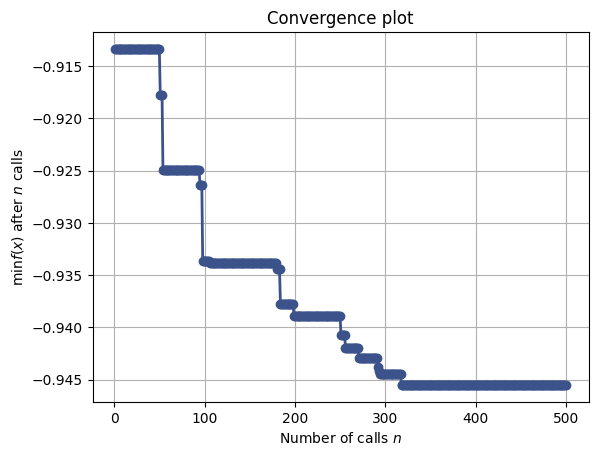
\includegraphics[width=\linewidth]{zernike_figures/convergence.png}
        \caption{Convergence plot}
    \end{subfigure}
    \hfill
    \begin{subfigure}{0.48\textwidth}
        \centering
        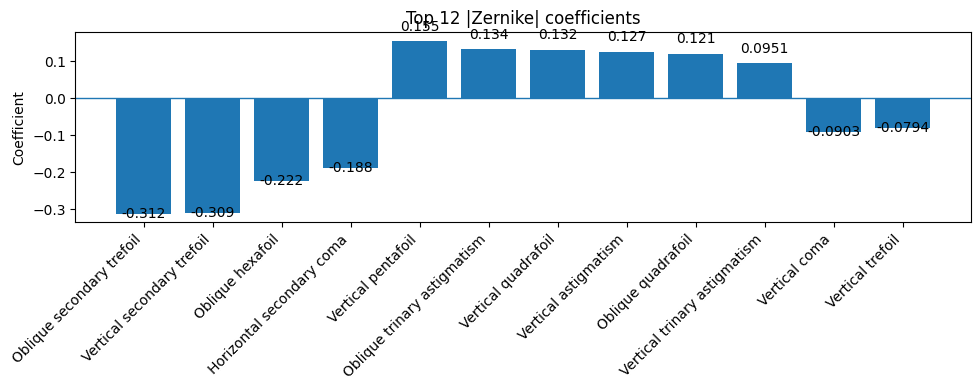
\includegraphics[width=\linewidth]{zernike_figures/zernike_coeffs.png}
        \caption{Optimal Zernike coefficients}
    \end{subfigure}
    
    % Row 2
    \begin{subfigure}{0.48\textwidth}
        \centering
        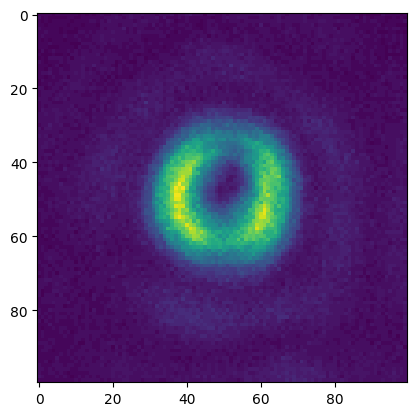
\includegraphics[width=\linewidth]{zernike_figures/bottle_before.png}
        \caption{Bottle beam before correction}
    \end{subfigure}
    \hfill
    \begin{subfigure}{0.48\textwidth}
        \centering
        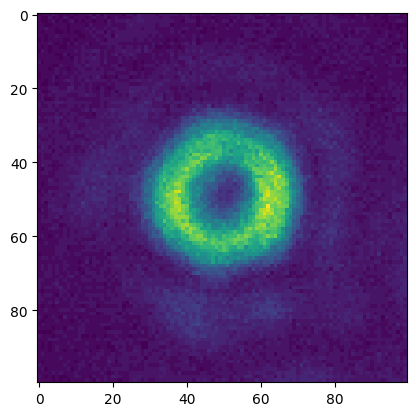
\includegraphics[width=\linewidth]{zernike_figures/bottle_after.png}
        \caption{Bottle beam after correction}
    \end{subfigure}
    
    \caption{Results of aberration correction using GP-UCB on 50 Zernike polynomials. (a) Convergence of best $R^2$ over iterations. improvevement of +3\% (b) Optimal Zernike coefficients found. (c) Intensity profile of bottle beam before correction. (d) Intensity profile of bottle beam after correction showing improved uniformity and symmetry.}
    \label{fig:aberration_results}
\end{figure}


\begin{figure}[ht]
    \centering
    % Row 1: Bottle beam fits
    \begin{subfigure}{0.48\textwidth}
        \centering
        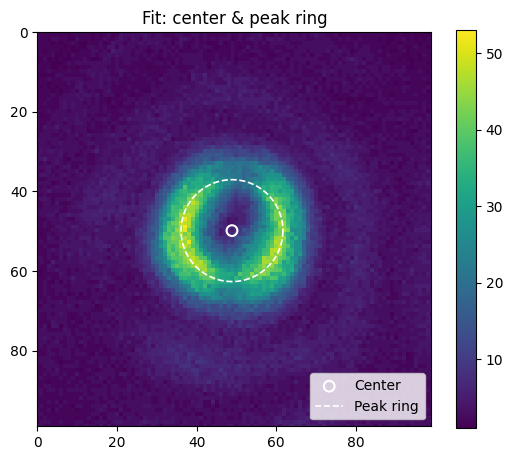
\includegraphics[width=\linewidth]{zernike_figures/bottle_before_fit.png}
        \caption{Bottle beam fit (before correction).}
        \label{fig:bottle_before_fit}
    \end{subfigure}
    \hfill
    \begin{subfigure}{0.48\textwidth}
        \centering
        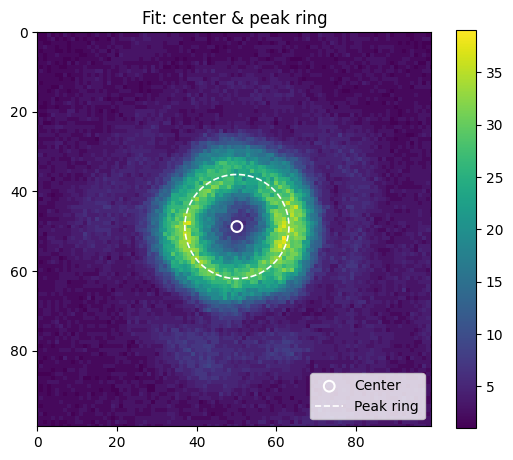
\includegraphics[width=\linewidth]{zernike_figures/bottle_after_fit.png}
        \caption{Bottle beam fit (after correction).}
        \label{fig:bottle_after_fit}
    \end{subfigure}

    % Row 2: Radial profiles
    \begin{subfigure}{0.48\textwidth}
        \centering
        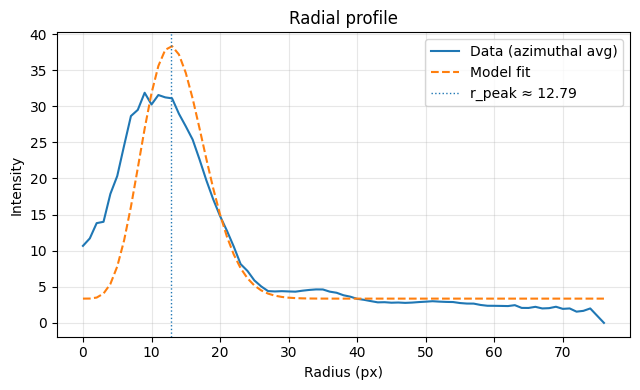
\includegraphics[width=\linewidth]{zernike_figures/radial_before.png}
        \caption{Radial intensity profile (before correction).}
        \label{fig:radial_before}
    \end{subfigure}
    \hfill
    \begin{subfigure}{0.48\textwidth}
        \centering
        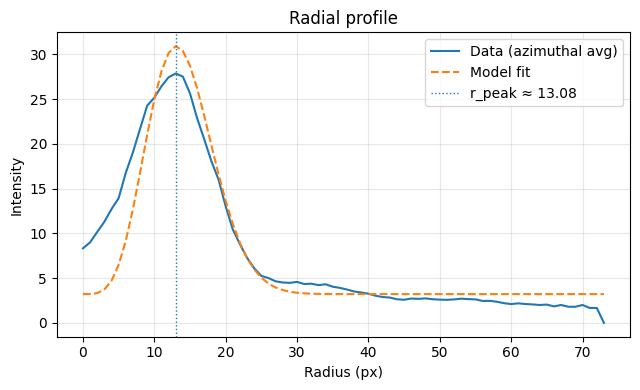
\includegraphics[width=\linewidth]{zernike_figures/radial_after.png}
        \caption{Radial intensity profile (after correction).}
        \label{fig:radial_after}
    \end{subfigure}

    % Row 3: Ring scans
    \begin{subfigure}{0.48\textwidth}
        \centering
        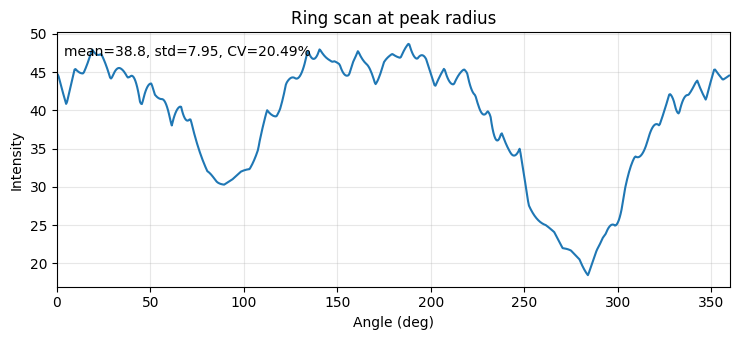
\includegraphics[width=\linewidth]{zernike_figures/ringscan_before.png}
        \caption{Ring scan at peak radius (before).}
        \label{fig:ringscan_before}
    \end{subfigure}
    \hfill
    \begin{subfigure}{0.48\textwidth}
        \centering
        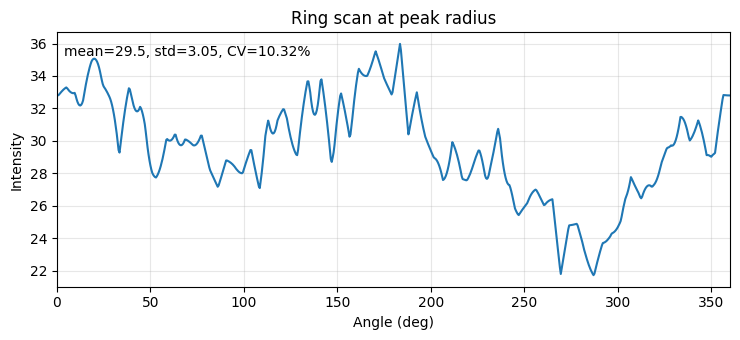
\includegraphics[width=\linewidth]{zernike_figures/ringscan_after.png}
        \caption{Ring scan at peak radius (after).}
        \label{fig:ringscan_after}
    \end{subfigure}

    % Row 4: X-scans
    \begin{subfigure}{0.48\textwidth}
        \centering
        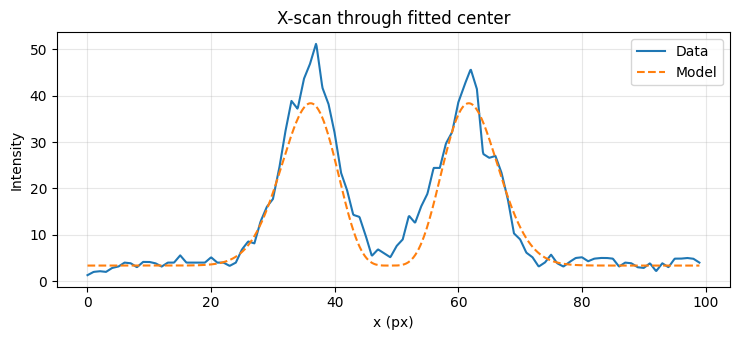
\includegraphics[width=\linewidth]{zernike_figures/xscan_before.png}
        \caption{X-scan through fitted center (before).}
        \label{fig:xscan_before}
    \end{subfigure}
    \hfill
    \begin{subfigure}{0.48\textwidth}
        \centering
        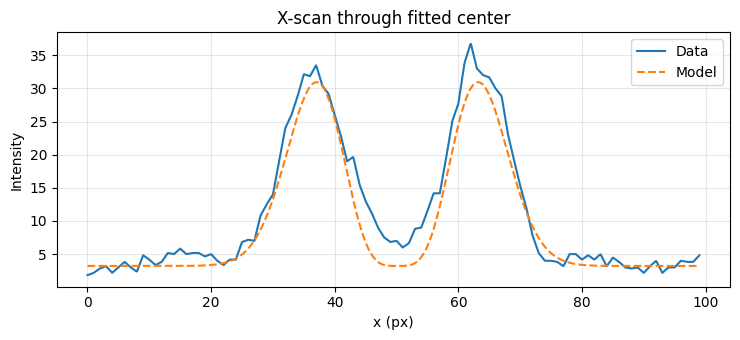
\includegraphics[width=\linewidth]{zernike_figures/xscan_after.png}
        \caption{X-scan through fitted center (after).}
        \label{fig:xscan_after}
    \end{subfigure}

    % Row 5: Y-scans
    \begin{subfigure}{0.48\textwidth}
        \centering
        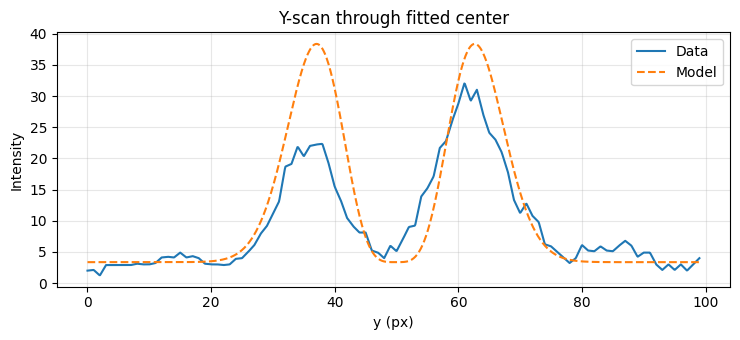
\includegraphics[width=\linewidth]{zernike_figures/yscan_before.png}
        \caption{Y-scan through fitted center (before).}
        \label{fig:yscan_before}
    \end{subfigure}
    \hfill
    \begin{subfigure}{0.48\textwidth}
        \centering
        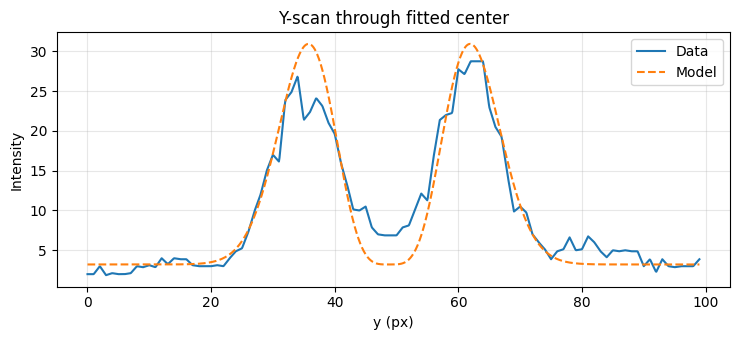
\includegraphics[width=\linewidth]{zernike_figures/yscan_after.png}
        \caption{Y-scan through fitted center (after).}
        \label{fig:yscan_after}
    \end{subfigure}

    \caption{Comparison of fitted profiles and line scans before and after aberration correction. 
    (a–b) Fitted bottle beams, (c–d) radial profiles, (e–f) ring scans, (g–h) x-scans, and (i–j) y-scans. 
    Correction improves radial symmetry and uniformity of the bottle beam.}
    \label{fig:profiles_line_scans}
\end{figure}










\end{document}
